
    \begin{center}
        \rule{20cm}{0.4pt} %линия {ширина линии}{высота}
    \end{center}
    \begin{multicols}{2}
        \begin{flushleft}
        \huge\textbf{{Метод\\ наименьших квадратов}}
        \end{flushleft}
        
        Метод наименьших квадратов применяется при обработке измерений для сглаживания <<шума>> эксперимента: этот метод позволяет исправлять случайные ошибки, неизбежно возникающие при изменениях, в том случае, когда характер зависимости измеряемой величины от независимой переменной задан.
        
        Рассмотрим простейшую ситуацию, когда измеряемая величина y зависит л\,и\,н\,е\,й\,н\,о о\,т о\,д\,н\,о\,й переменной x. Пусть произведено n измерений и для значений $x_1, x_2, \ldots, x_n$ переменной x получены замеры $y_1,y_2,\ldots ,y_n$. З\,а\,д\,а\,ч\,а состоит в проведении прямой $y=ax+b$, наилучшим образом прилегающей к точкам $P(x_1;y_1), P(x_2;y_2), \ldots,P(x_n;y_n)$. %\, сжатый пробел
        
        Решение задачи, разумеется, зависит от того, что понимается под словами <<наилучшим образом прилегающей>>. Суть метода наименьших квадратов (его называют так же методом Гаусса) состоит в том, что <<наилучшей>> считается та прямая, для которой принимает наименьшее значение сумма квадратов отклонений, т. е. выражение
        \begin{equation}
         A_n = \sum\limits_{i=1}^n(y_i - (ax_i)+b))^2 .
        \end{equation}

        
        На рисунке изображена искомая прямая $y = ax+b$ и точки $P_1, \ldots, P_n$. Разность 
        $y_i - (ax_i +b)$ показывает отклонение (вдоль оси ординат) экспериментальной точки $P_i(x_i,y_i)$ от искомой прямой.
        
        Как найти значение a и b, минимизирующие выражения (1)? Предположим, что такие значения существуют, и параметр a нами уже найден. Чтобы найти b, перепишем $A_n$ в виде
        \begin{flushright}
         $A_n = \sum\limits_{i=1}^n (y_i -ax_y)^2 - \sum\limits_{i=1}^n 2b(y_i - ax_i) +$\\
        $+\sum\limits_{i=1}^n b^2 = n*b^2 -2b \sum\limits_{i=1}^n (y_i - ax_i) +$\\
	    $+\sum\limits_{i=1}^n (y_i - ax_i)^2.$
	    \end{flushright}
	    
        \begin{flushleft}
        
	    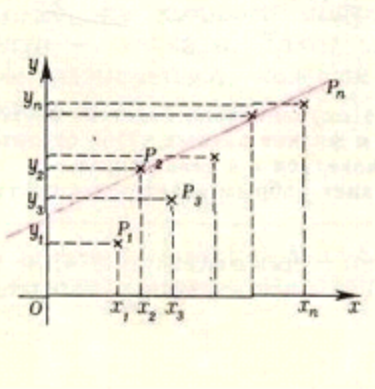
\includegraphics[scale=0.5]{Рисунок 1.PNG} %умножает размеры изображения на коэффициент
	    \end{flushleft}


	    Рассмотрим $A_n$ как (квадратичную) функцию от b. Она достигает минимума при 
	    \begin{flushleft}
	    $b = \frac{1}{n}\sum\limits_{i=1}^n (y_i - ax_i) =$
	    \end{flushleft}
	    \begin{flushright}
	    $=\frac{1}{n}\sum\limits_{i=1}^n y_i - \frac{a}{n}\sum\limits_{i=1}^n x_i .$
	    \end{flushright}
	    Положив 
	    $$\bar x  = \frac{1}{n}\sum\limits_{i-1}^n x_i ;\; \bar y = \frac{1}{n}\sum\limits_{i=1}^n y_i$$\\ %\; еще вид пробела. Чуть больше 
	    можно написать $b = \bar y - a\bar x$, откуда для $A_n$ получим\\
	    $A_n = \sum\limits_{i=1}^n ((y_i - \bar y) - a(x_i - \bar x))^2 =$
	    \begin{center}
	    $=a^2\sum\limits_{i=1}^n (x_i - \bar x)^2 -$\\
	    $-2a \sum\limits_{i=1}^n (y_i - \bar y) (x_i - \bar x) + \sum\limits_{i=1}^n (y_i - \bar y)^2 .$
	    \end{center}
	    Рассмотрим теперь $A_n$ как квадратичную функцию от a. Она очевидно достигает минимума при \\ 
	    $a = \sum\limits_{i=1}^n (y_i - \bar y)(x_i - \bar x) \bigg/ \sum\limits_{i=1}^n (x_i - \bar x)^2 .$\\ 
	    Наилучшей оказалась прямая $y=ax+b$, где 
	    \begin{center}
	    $a=\frac{ \sum\limits_{i=1}^n (y_i - \bar y)(x_i - \bar x)}{\sum\limits_{i=1}^n (x_i - \bar x)^2}$
	    $b = \bar y - \frac{ \bar x \sum\limits_{i=1}^n (y_i - \bar y)(x_i - \bar x)}{\sum\limits_{i=1}^n (x_i - \bar x)^2}$
	    \end{center}
	    
	    Задачи
	    \begin{enumerate}
	        \item Решить задачу о сглаживании шума методом Гаусса для следующих не линейных функций от одной переменной
	        \begin{enumerate}
	            \item $y=ax^2+bx+c;$
	            \item $y = a\cdot \cos x + b \cdot \sin x .$
	        \end{enumerate}
	        \item Как <<работает>> метод Гаусса в пространстве (для двух независимых переменных)? Рассмотрите задачу для плоскости $z = ax +by +c *)$
	        \item Найти точку, для которой 
	        \begin{enumerate}
	            \item сумма расстояний от трех заданных точек (не лежащих на одной прямой) минимальна;
	            \item задача 3а) - для n точек, не лежащих на одной прямой;
	            \item сумма расстояний от трех заданных окружностей минимальна.
	        \end{enumerate}
	    \end{enumerate}
	    \begin{flushright}
	    А. Строгова
	    \end{flushright}
	    \begin{center}
        \rule{280 pt}{0,4 pt} %линия
        \end{center}
	    \par *) Геометрическая иллюстрация к этой задаче дана на первой полосе обложки <<Кванта>> № 8.
    \end{multicols}

    \begin{table}
    \hspace{393 pt}
    \bf{Таблица 1}
    \begin{center}
    \begin{tabular}{|*{9}{c|}} \hline
    $|\Delta K|$ & $h_6$ & $h_M$ & $|\Delta K|$ & $h_6$ & $h_M$ & $|\Delta K|$ & $h_6$ & $h_M$ 
    \\ \hline 
    0-3 & 50 & 50 & 122-129 & 67 & 33 & 279-290 & 84 & 16 \\ \hline
    4-10 & 51 & 49 & 130-137 & 68 & 32 & 291-302 & 85 & 15 \\ \hline
    11-17 & 52 & 48 & 138-145 & 69 & 31 & 303-315 & 86 & 14 \\
    18-25 & 53 & 47 & 146-153 & 70 & 30 & 316-328 & 87 & 13 \\
    26-32 & 54 & 46 & 154-162 & 71 & 29 & 329-344 & 88 & 12 \\
    33-39 & 55 & 45 & 163-170 & 72 & 28 & 345-357 & 89 & 11 \\
    40-46 & 56 & 44 & 171-179 & 73 & 27 & 358-374 & 90 & 10 \\
    47-53 & 57 & 43 & 180-188 & 74 & 26 & 375-391 & 91 & 9 \\
    54-61 & 58 & 42 & 189-197 & 75 & 25 & 392-411 & 92 & 8 \\
    62-68 & 59 & 41 & 198-206 & 76 & 24 & 412-432 & 93 & 7 \\
    69-76 & 60 & 40 & 207-215 & 77 & 23 & 433-456 & 94 & 6 \\
    77-83 & 61 & 39 & 216-225 & 78 & 22 & 457-484 & 95 & 5 \\
    84-91 & 62 & 38 & 226-235 & 79 & 21 & 485-517 & 96 & 4 \\
    92-98 & 63 & 37 & 236-245 & 80 & 20 & 518-559 & 97 & 3 \\
    99-106 & 64 & 36 & 246-256 & 81 & 19 & 560-619 & 98 & 2 \\
    107-113 & 65 & 35 & 257-267 & 82 & 18 & 620-735 & 99 & 1 \\
    114-121 & 66 & 34 & 268-278 & 83 & 17 & свыше 735 & 100 & 0
    \\ \hline 
    \end{tabular}
    \end{center}
    \end{table}


